\pgfplotsset{width=8cm,compat=1.14}
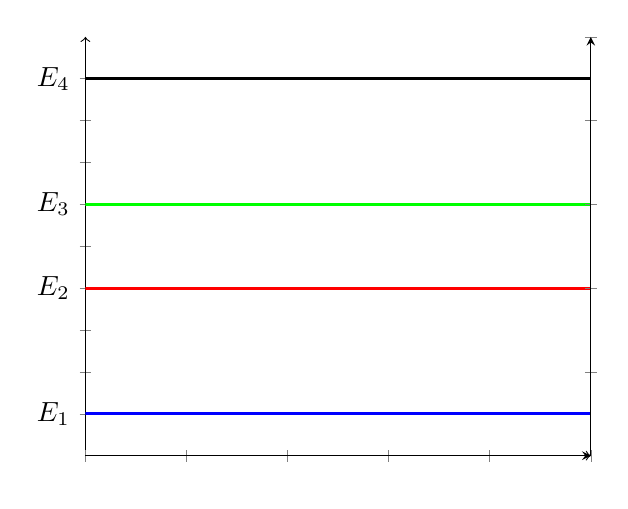
\begin{tikzpicture}
    \begin{axis}
        [
        axis lines=middle,
        axis line style={->},
        xmin=0,
        xmax=5,
        xticklabels={,,},
        ymin=0,
        ymax=10,
        ytick={0,1,...,9},
        yticklabels={,$E_1$,,,$E_2$,,$E_3$,,,$E_4$},
        ylabel near ticks,
        ]
        \addplot[blue, very thick,samples=200,domain=0:5] {1};
        \addplot[red, very thick,samples=200,domain=0:5] {4};
        \addplot[green, very thick,samples=200,domain=0:5] {6};
        \addplot[black, very thick,samples=200,domain=0:5] {9};
    \end{axis}
    \begin{axis}
        [
        xshift=0cm,
        axis lines=middle,
        xticklabels={,,},
        ymin=0,
        ymax=10,
        yticklabels={,,},
        xmin=-5,
        xmax=0,
        ]
    \end{axis}
\end{tikzpicture}
